% STAGED 2026-09-25. These are the only Xi figures proposed for restoration.
% The older xiFrameGeo/xiBalance/xiWrapLoss figures remain dropped.

% INSERT after the paragraph that introduces the local bracket frame.
For the two-rotation evaluator, the bracket frame was constructed from the vector joining the bracket origin to attachment point $\mathbf{p}_{A}$ or $\mathbf{p}_{B}$. The first rotation, through $\theta_z$ about the fixed space-frame axis $\hat z_s$, points the intermediate axis $\hat x_1$ toward the sagittal-plane projection $\mathbf{p}_{A/B}^{\mathrm{sag}}$. The second rotation, through $-\theta_y$ about the current axis $\hat y_1=\hat y_{br}$, brings the final bracket axis $\hat x_{br}$ into alignment with the full three-dimensional point vector. Figure~\ref{fig:xiFrameTransform} shows these geometric targets. The resulting orientation and homogeneous transform are

\begin{equation}
\mathbf{R}_{s,br}=\mathbf{R}_z(\theta_z)\mathbf{R}_y(\theta_y)^T,
\qquad
{}^{s}\mathbf{T}_{br}=
\begin{bmatrix}
\mathbf{R}_{s,br} & \mathbf{p}_{br}\\
\mathbf{0}^{T} & 1
\end{bmatrix}.
\label{eq:bracket_frame_transform}
\end{equation}

\begin{figure}[htbp]
\centering
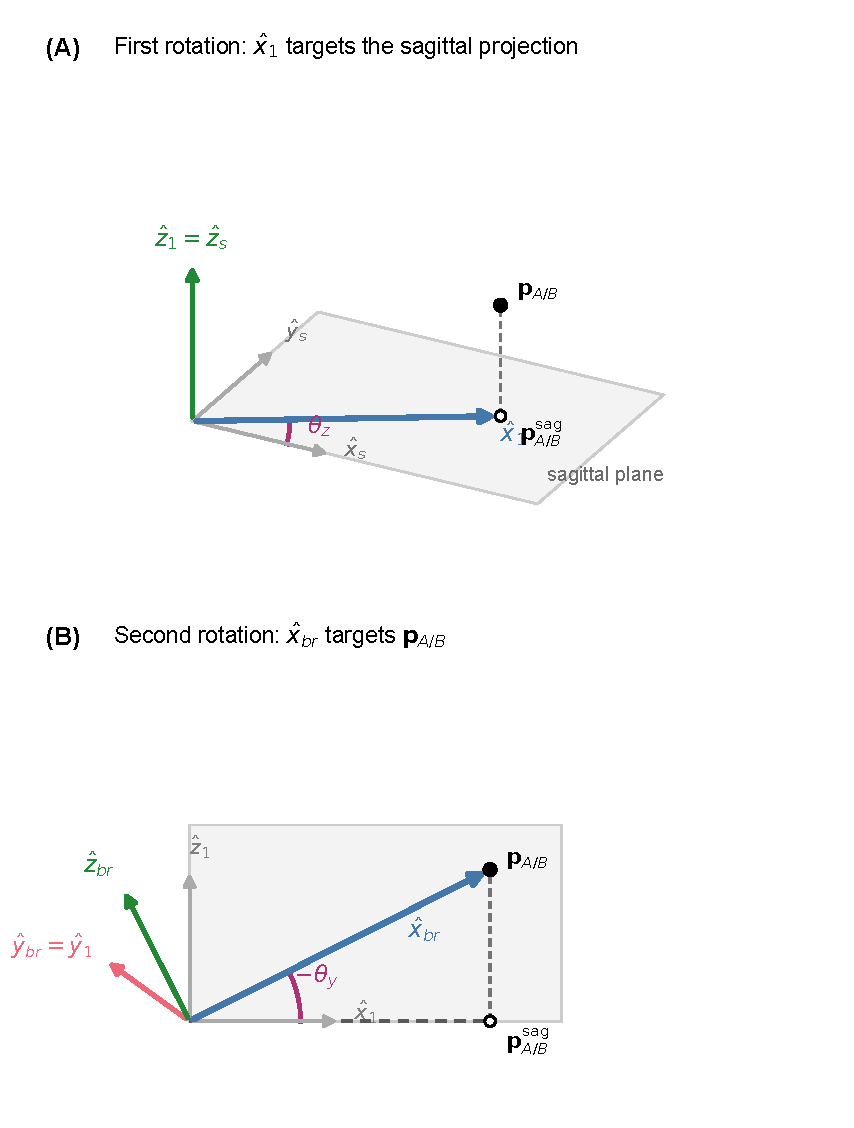
\includegraphics[height=0.72\textheight]{xiFrameTransform.pdf}
% ALT TEXT: Two vertically stacked diagrams construct the local bracket frame.
% Panel A rotates about the fixed space z axis until the intermediate x axis
% points toward the sagittal-plane projection of attachment point pA or pB.
% Panel B rotates about the current y axis until the final bracket x axis points
% directly toward the full three-dimensional attachment point.
\caption[Two-rotation construction of the bracket frame]{Two-rotation construction of the bracket frame from attachment point $\mathbf{p}_{A}$ or $\mathbf{p}_{B}$. \textbf{(A)} Rotation through $\theta_z$ about fixed $\hat z_s$ aligns $\hat x_1$ with the point's sagittal-plane projection. \textbf{(B)} Rotation through $-\theta_y$ about current $\hat y_1=\hat y_{br}$ aligns $\hat x_{br}$ with the full point vector.}
\label{fig:xiFrameTransform}
\end{figure}

% INSERT after Equation~\ref{eq:bktcomponentdeflection}. Update the surrounding
% equation notation from epsilon to eta so epsilon remains available elsewhere.
Figure~\ref{fig:xiProjection} distinguishes the three-dimensional displacement of each bracket from the scalar displacement along the BPA force path. For bracket $j$, the displacement resolves into components $\eta_{1,j}$, $\eta_{2,j}$, and $\eta_{3,j}$ along the local bracket-frame basis, whereas only its projection $\delta_{br,j}$ along the corresponding force direction $\hat{\mathbf{u}}_j$ changes the actuator length. The two bracket projections act in series with the tendon elongation $\delta_{\mathrm{tendon}}$.

\begin{equation}
\begin{aligned}
\boldsymbol{\eta}_{br,j} &= \sum_{i=1}^{3}\eta_{i,j}\hat{e}_i^{(j)},\\
\delta_{br,j} &= \hat{\mathbf{u}}_j^T\boldsymbol{\eta}_{br,j}, \qquad j\in\{1,2\},\\
\delta_{\mathrm{series}} &= \delta_{br,1}+\delta_{\mathrm{tendon}}+\delta_{br,2}.
\end{aligned}
\label{eq:bracket_series_projection}
\end{equation}

\begin{figure}[htbp]
\centering
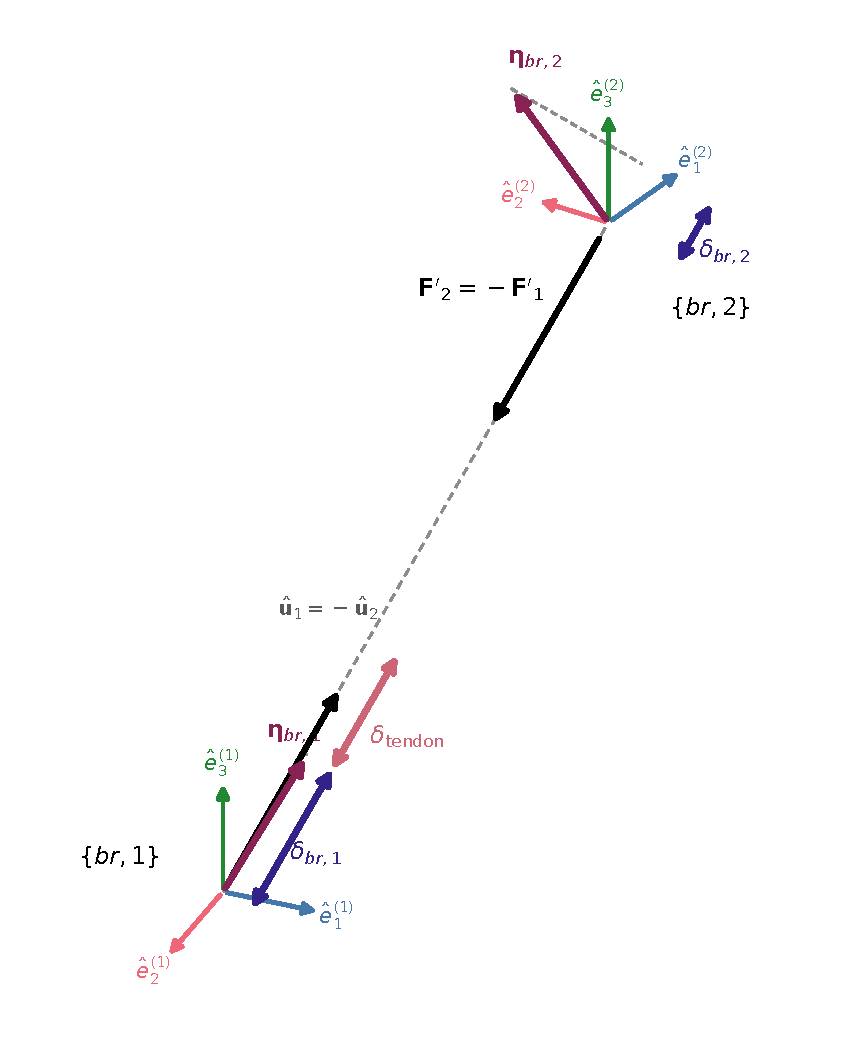
\includegraphics[height=0.72\textheight]{xiProjection.pdf}
% ALT TEXT: Two three-dimensional bracket coordinate frames, {br,1} and {br,2}, are
% separated along a dashed actuator line. Equal-and-opposite force vectors point
% from each bracket toward the other and satisfy F'_2=-F'_1. Each bracket has a local deflection vector
% eta and a clearly offset scalar projection delta along its force direction. The
% bracket-2 projection is shifted to the right of its coordinate axes. Tendon
% elongation delta_tendon is collinear and contiguous with the bracket-1 projection.
\caption[Two-bracket deflection and force-path projection]{Two-bracket deflection and projection along the BPA force path. The force vectors at $\{br,1\}$ and $\{br,2\}$ point toward one another and satisfy $\mathbf{F}'_2=-\mathbf{F}'_1$. The bracket projections $\delta_{br,1}$ and $\delta_{br,2}$ are offset from the corresponding coordinate frames for clarity, and tendon elongation $\delta_{\mathrm{tendon}}$ continues collinearly from $\delta_{br,1}$. Colors follow a color-vision-deficiency-safe palette and are redundant with labels and line weights.}
\label{fig:xiProjection}
\end{figure}
